\renewcommand{\chaptername}{Diseño de un puente H para el posicionador}
\graphicspath{{parte_4/puente_h/}}
\chapter{Diseño de un puente H para el posicionador} \label{cap:driver_motores}
\markright{Diseño de un puente H para el posicionador} 
\begin{center}
	\begin{tcolorbox}[colback=gray!5!white, %Color del fondo
		colframe=blue!75!black,
		title= \center{\Large{Resumen}} ]
		En esta sección, se diseña y seleccionan los componentes electrónicos para controlar los motores que mueven la antena. El circuito que se realiza es el denominado puente H, el cual permite la inversión de polaridad para poder mover la antena en ambos sentidos. 
	\end{tcolorbox}
\end{center}    


\section{introducción}
	
	Se realiza el diseño y construcción de un puente H basado en transistores mosfet de canal P y canal N. Se realiza de esta manera dado que se dispone de una única fuente de alimentación, y al usar ambos tipos de transistores, no es se necesita elevar la tensión respecto de la tensión de alimentación para realizar el disparo de los mosfet. Los mosfet seleccionados son el IRFP240 (canal N) y el IRF 9530(canal P) ambos disponibles en el mercado local. Estos mosfet se han seleccionado por poder manejar las corrientes del motor que mueve la antena. En total se realizan dos puentes H, uno para cada motor y, por tanto, se muestra el análisis de uno solo de estos, ya que el otro circuito es idéntico.Se debe proteger cada puente H contra el cortocircuito debido a que los pines del microcontrolador se ponen en nivel bajo al cargar un código. Por tanto, se diseñan dos circuitos de control para el puente H, y luego se elige el diseño que se adapta a la hoja de datos de los transistores mosfet. También, se selecciona el disipador para el uso adecuado de los transistores mosfet, ya que deben evacuar el calor generado en su interior.  
	
	
\section{Análisis de los transistores Mosfet y BJT} 

Se analiza el funcionamiento de los transistores MOSFET y BJT cuando son usados como llave on/off. En general los MOSFET tienen rápida respuesta (del orden de nanosegundos), y soportan varios ampere de corriente. Estos, se usan para dirigir el sentido de giro de un motor, en una estructura conocida como puente H. Este circuito, permite invertir el sentido de la corriente, y con esto logra cambiar el sentido de giro de los motores (o visto de otro modo, invierte la polaridad de la tensión sobre la carga). 

Los transistores mosfet, son controlados por transistores BJT de propósito general. Estos, realizan el accionado de dejar pasar o no la corriente sobre los transistores mosfet. Estos transistores, se comandan desde el microcontrolador.
 
%A continuación, se da una breve descripción de los transistores MOSFET y BJT, y en la sección siguiente, se muestran las características particulares de los dispositivos mosfet y BJT seleccionados.
%
\subsection{Transistor Mosfet} 

El transistor de tipo mosfet se basa en tres terminales, llamados Gate, Source y Drain. Existen dos tipos: incrementales (o de enriquecimiento) y decrementales (o decrecimiento). El mosfet de tipo decremental no se utiliza, y por tanto, solamente se hace mención de él. El tipo de mosfet utilizado es el incremental. 

El mosfet incremental (válido para el decremental también), se denominan de canal N o de canal P. Se brinda la explicación sobre el mosfet de canal N, y el de canal P, se deben invertir las polaridades de tensión. En el mosfet de canal N, basa su funcionamiento en que al existir una tensión entre Gate y Source positiva, más alta que una tensión denominada ``tensión umbral''($V_{t}$) el dispositivo mosfet, empieza a conducir, en una zona de operación llamada de saturación. El diagrama de un mosfet es el que muestra la figura \ref{fig:mosfet_str_model}. No se dan las explicaciones sobre la física del dispositivo de estado sólido, pero se ilustra a continuación en conjunto con el circuito de prueba: 

\begin{figure}[ht!]
	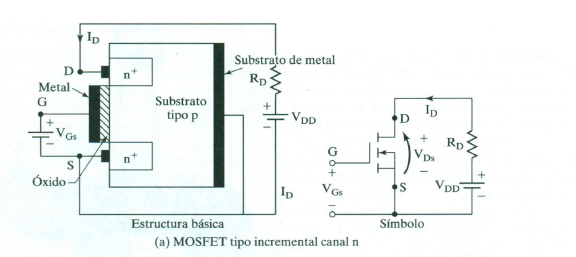
\includegraphics{mosfet_estr}
	\caption{Esquema de un mosfet a la izquierda. A la derecha se muestra el modelo circuital y su símbolo}
	\label{fig:mosfet_str_model}
\end{figure}

Si se realiza el circuito de la derecha sobre un mosfet de canal N, se obtienen las siguientes curvas:

\begin{figure}[ht]
	\begin{subfigure}{0.5\linewidth}
		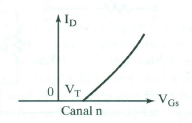
\includegraphics[width=\linewidth]{curva_1_mosf}
		\caption{Gráfica $V_{gs}$ vs $ I_d$}
	\end{subfigure}
	\hfil
	\begin{subfigure}{0.5\linewidth}
		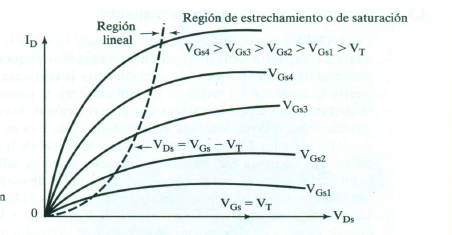
\includegraphics[scale=0.75]{curva_2_mosf}
		\caption{Gráfica $V_{ds}$ vs $ I_d$ con $V_{gs}$ constante}
		\label{fig:vds_vs_id_mosfetop}	
	\end{subfigure}
\caption{Curvas características de un transistor mosfet de canal N}
\end{figure}

Donde $V_t$ es la tensión umbral del dispositivo. Se observa en la curva \ref{fig:vds_vs_id_mosfetop} que existen tres regiones de operación del mosfet, estas son:
\begin{enumerate}
	\item Región de corte: ocurre cuando $V_{gs}<V_t$. En esta condición la corriente entre Drain y Source es nula, es decir, se tiene una llave abierta.
	\item  Región de saturación: en esta zona se cumple la siguiente desigualdad: $V_{gs}>V_t$ y $V_{gs}-V_{t}<V_{ds}$. En esta zona se tiene la saturación y la llave se comporta como una fuente de corriente controlada por tensión. 
	\item Región óhmica o zona óhmica: en este caso se tiene la siguiente desigualdad: $V_{gs}>V_t$ y $V_{gs}-V_t>V_{ds}$. El dispositivo permite el paso de corriente entre los terminales drain y source. 
\end{enumerate} 

En la zona óhmica, se presenta una resistencia, llamada $R_{ds}$ cuando empieza a conducir el mosfet. Este valor viene dado por la pendiente de la recta en la zona óhmica. Esta pendiente esta dada por:
\begin{equation*}
	R_{ds} =\frac {V_{gs}}{I_{ds}} 
\end{equation*}

Se utiliza la zona óhmica, debido a que la corriente que circula por la carga es variable, y se debe fijar la tensión entre Gate y Source. Por este motivo, para el diseño del puente H,se trabaja en  esta zona. 

\subsection{Transistor BJT como llave electrónica} \label{sub:bjt_llave}

El transistor BJT es un transistor que tiene tres junturas, de tipo NPN y PNP. Este dispositivo puede usarse como llave electrónica o para la amplificación de señales (zona activa). Para este trabajo, se usa como llave, y se explica su funcionamiento en esta zona, dejando de lado la zona activa de los transistores. El símbolo del transistor es el siguiente: 
\vspace{-5mm}
\begin{figure}[h]
	\begin{subfigure}{0.5\textwidth}
		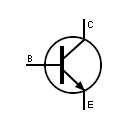
\includegraphics{simbol_npn}
		\caption{símbolo del transistor BJT de tipo NPN }
	\end{subfigure}
	\hfill 
	\begin{subfigure}[h]{0.5\textwidth}
		
\includegraphics{simbol_pnp}
		\caption{símbolo del transistor BJT de tipo PNP }
	\end{subfigure} 
\caption{Símbologia electrica de transistores BJT} 
\end{figure}
\vspace{-5mm}

En la figura anterior, se ven dos tipos de transistores NPN y PNP. En ella se observa que es un dispositivo de tres terminales, denominados emisor(E) – base(B) y colector (C).  

Debido a que tiene tres terminales,se las puede asociar a un tipo de juntura NP o PN, y en base a la polarización de estas, se  determina el uso del transistor. Estas junturas son colector – base y base-emisor. En el caso de un transistor NPN, la juntura colector base es de tipo NP, y la juntura Base – emisor es de tipo PN. 

El transistor PNP o NPN, poseen distintas configuraciones según sean los circuitos de configuración (topología del circuito): emisor común – base común y colector común. En esta sección, solo se considera la topología emisor común, ya que es la que se usa en este trabajo. Esta topología, usa al transistor como llave on/off.  

Los transistores BJT, ya sean PNP o NPN, tienen un conjunto de curvas características, que determinan como es la transferencia entre los parámetros del transistor. Estas curvas, se muestran en la figura \ref{fig:curvas_bjt} para el transistor de tipo NPN. Si desea las curvas del transistor PNP, basta con invertir las tensiones: 

\begin{figure}[h!]
	%\centering 
	\begin{subfigure}{0.4\linewidth}
		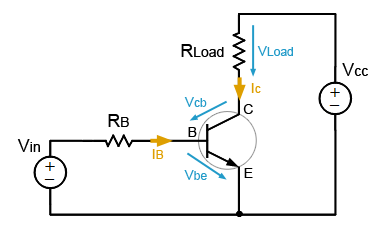
\includegraphics[scale=0.5]{curva_entrada_bjt}
		\caption{Curva característica de entrada}
		\label {fig:circ_pol_bjt}
	\end{subfigure}
\hspace{15mm}
	\begin{subfigure}{0.4\linewidth}
		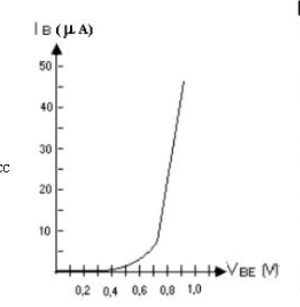
\includegraphics[scale=0.5]{curva_entrada_bjt_1}
		\caption{Circuito característico en topologia emisor común para obtener las curvas características}
		\label{fig:ib_vs_vbe}
	\end{subfigure}
\begin{center}
	\hspace{-25mm}
	\begin{subfigure}{0.4\linewidth}
		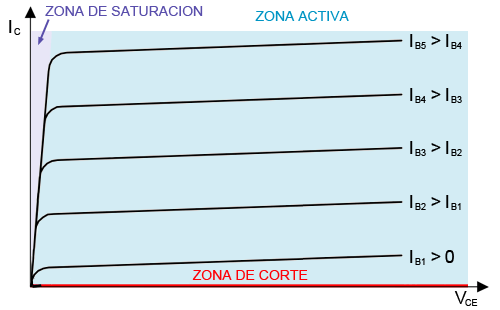
\includegraphics[scale=0.5]{Curva_ic_vs_vce}
		\caption{Curva característica regiones de operación de un transistor}
		\label{fig:Ic_vs_vce}
	\end{subfigure}
\end{center}
\caption{Curvas características de un transistor BJT}
\label{fig:curvas_bjt}
\end{figure}

Se observa en la figura \ref{fig:ib_vs_vbe} que la relación entre la corriente de base y la tensión base emisor (que es una juntura pn en este caso), se comporta como si fuese un diodo.  En la figura \ref{fig:Ic_vs_vce} se observa que el transistor tiene tres regiones de operación: saturación – activa y corte. La zona de corte, ocurre cuando la corriente de base es nula. En la región activa, la corriente de colector es proporcional a la corriente de base. Este factor de proporción se denomina ``ganancia del transistor'', y se lo denota con $\beta$ o con $h_{FE}$, y son un parámetro individual de cada transistor. En otras palabras, en la zona activa se cumple: 
\begin{equation} \label{eq:bjt_zona_act}
	I_c = \beta I_b
\end{equation}

En la zona de saturación, se observa (ver figura \ref{fig:Ic_vs_vce}) que la relación no se cumple, es más, se observa que la relación entre la corriente de base a colector es mayor que la de colector entre la ganancia del transistor. En otras palabras, se cumple que: 	

\begin{equation}
	I_b > \frac{I_c}{\beta} 
\end{equation}

Cabe destacar, que esto ocurre por la polarización de la juntura. En el caso de corte, ambas junturas se polarizan en inversa, y en saturación, ambas se polarizan en directa. En este estado, la tensión $V_{ce}$ de la figura \ref{fig:circ_pol_bjt} es muy pequeña, polarizando entre colector y base de forma directa. Si la juntura Base emisor se polariza en polarización directa, mientras la juntura entre colector y base en polarización inversa, se está en zona activa (es decir, en la zona de amplificación y se cumple la ecuación \ref{eq:bjt_zona_act}). 

Por las gráficas de la figura \ref{fig:curvas_bjt}, se observa que la zona de trabajo de un transistor depende fuertemente de la corriente de base, y la topología de circuito que se esté utilizando. Por ello, es que es necesario, determinar dos parámetros importante: resistencia de base($R_B$ en la figura \ref{fig:circ_pol_bjt}) y máxima corriente de colector en zona activa Este parámetro, permite determinar si el transistor se satura o no, pues es necesario elevar la corriente de base por encima de una valor mínimo para que el transistor entre en saturación.  
Para calcular la resistencia de base, se analiza el circuito que está a continuación: 


\begin{figure}[ht!]
	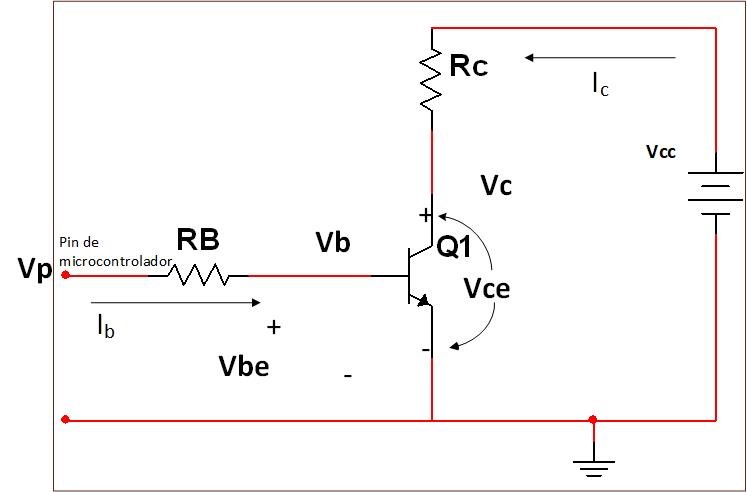
\includegraphics[scale=0.8]{circuito_analisisBJT} 
	\caption{Circuito para el cálculo de la resistencia de base de un transistor bipolar NPN. En este diagrama donde dice ``pin de microcontrolador'' es el control del transistor entre corte y saturación realizado mediante la programación del sistema embebido}
	\label{fig:calc_RB}
\end{figure}


De la figura \ref{fig:calc_RB}, donde dice ``pin del microcontrolador'', es el pin destinado a poner en corte al transistor, o saturarlo. Dada una resistencia de colector ($R_c$ en figura \ref{fig:calc_RB}), y una tensión de entrada $V_p$ (ver figura \ref{fig:calc_RB}), se  obtienen las ecuaciones para el cálculo de $R_B$. 
Si realizamos la malla entre colector y emisor, cerrándola sobre el mismo transistor, se tiene la siguiente ecuación de Kirchhoff: 

\begin{equation} \label{eq:state_bjt}
	V_{CE} = V_{BE} + V_{CB} \rightarrow V_{CB}= V_{CE} - V_{BE}
\end{equation}

Para que el transistor se encuentre en estado de corte, se debe cumplir que $V_{CB}>0$  y la tensión $V_{BE}<0$ o menor a un valor que especifique el fabricante del dispositivo (generalmente 0.6V), la saturación se da cuando $V_{BE}>0$ y $V_{CB}<0$. Si un transistor cumple que $V_{CB}>0$ y $V_{BE}>0$, se puede afirmar (en base a la expresión \ref{eq:state_bjt}) $V_{CE}>V_{BE}$, y el transistor esta en zona activa.

Si suponemos el transistor en zona activa, de la expresión \ref{eq:state_bjt}, la corriente máxima de colector, la podemos obtener, igualando $V_{CB}=0$. Si esto ocurre, $I_C$  adopta el valor de (resolviendo la malla de la derecha de la figura \ref{fig:calc_RB}):
\begin{equation} \label{eq:ICmaxSat}
	I_{Cmax} = \frac{V_{CC} - V_{CE}}{R_c} = \frac{V_{CC} - V_{BE}}{R_c}
\end{equation} 

y el valor de la corriente de base para esta condición es: 
\begin{equation}\label{eq:IB_min}
	I_{Bmin} = \frac{I_{Cmax}}{\beta}
\end{equation}

Luego, si la corriente por la base, aumenta por encima de $I_{Bmin}$ , entonces $V_{BE} $ aumenta la corriente de colector, disminuyendo $V_{CE}$   y esta baja hasta un valor menor a $V_{BE}$. En este punto, la tensión $V_{CE}$ se denomina tensión colector-emisor de saturación, y la denotamos: $V_{CEsat}$. Para obtener la corriente de colector en estas condiciones: 
\begin{equation} \label{eq:IC_sat}
	I_{Csat} = \frac{V_{CC}- V_{CEsat}}{R_c} 
\end{equation}

Por tanto, dado una $I_{Bmin}$, la $I_{B}$ que circule por la base, debe ser mayor a esta $I_{Bmin}$. Con estos datos, podemos hallar una resistencia de base, que satisfaga estos requerimientos. De la figura \ref{fig:calc_RB}, usando la malla del lado izquierdo:
se obtiene que\footnote{Para llegar a esta expresión, se debe plantear que $I_{b}>I_{bmin}$ y despejar $R_B$}: 
\begin{equation} \label{eq:select_rb}
	R_B < \frac{V_p-V_{BE}}{I_{bmin}}
\end{equation} 

Luego, se debe seleccionar una $R_B$ que satisfaga la desigualdad anterior.%\ref{eq:select_rb}.  
Cuando la tension $V_p$ es cero, el transistor está cortado, y no hay circulación de corriente en la malla. En esta situación, ocurre que $V_{BE}=0$. Por ende, el procedimiento para seleccionar la resistencia, tanto de colector, como de base, se basa en las corrientes de base y colector. Estas, tienen valores máximos y mínimos brindados por los fabricantes, y se debe tener la hoja de datos al seleccionar esta resistencia. 

\subsection{Componentes seleccionados} 


Los mosfet se eligien de tal manera que cumplan tres requerimientos:
\begin{itemize}
	\item Disponibilidad en el mercado local 
	\item Menor resistencia entre Drain y source 
	\item Soporten una corriente variable entre 0.4 A y 7 A   
	
\end{itemize}
 
Los mosfet que se encuentran en el mercado local que cumplen todos los requisitos son el IRFP240(canal N) y el IRF9530(canal P). Una vez seleccionados, resta elegir la tensión entre gate y source para ambos dispositivos. Además, se eligieron dos de canal P y dos de canal N ya que se cuenta con una única fuente de tensión. 


\subsubsection{Mosfet IRFP240} \label{sub:irfp240}

Este mosfet es de canal N, con una $R_{ds}$ máxima de 0.18 ohm. Su tensión umbral $V_{t}$ oscila entre 2V y 4V. Por tanto, la tensión entre $V_{gs}$ debe ser superior a 4 volts para asegurar su conducción. Para decidir qué tensión se debe aplicar entre Gate y Source, se debe tener en cuenta, la tensión máxima que soporta entre gate y source ($V_{gs}$). Este dato, extraído de la hoja de datos es 20V. De la discusión precedente, obtenemos que $V_{gs}$ debe estar comprendida entre 4v y 20v (ver \cite{IRFP240}). 
Dado que la tensión entre gate y source está definida sobre un rango de tensiones, se debe elegir aquella que minimice la resistencia entre Drain y source ($R_{ds}$), y tenga un rango de operación completo entre 7 Ampere y 0.44 Ampere (corriente consumida por el motor). La curva $I_d$ a $V_{gs}$ a una temperatura de 25° C se obtiene del datasheet, y se muestra en la figura \ref{fig:irfp_240_id_vs_vds}: 

\begin{figure}[ht!]
	\centering
	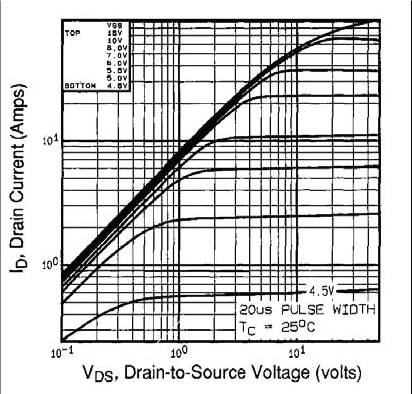
\includegraphics{curva_datasheet_1} 
	\caption{Diagrama de Id vs Vgs del mosfet IRFP240. Esta curva la brinda el fabricante, para distintos valores de Vgs}
	\label{fig:irfp_240_id_vs_vds}
\end{figure}

De la figura anterior(\ref{fig:irfp_240_id_vs_vds}) se observa que la tensión $V_{gs}$ más chica es de 4.5 V, y se obtiene una corriente máxima de aproximadamente 0.5 Ampere. La curva siguiente, se tiene $V_{gs}$ de 5V, y una corriente máxima de 2.3 Ampere aproximadamente. La que sigue, tiene una tensión de 5.5 V y una corriente de 6 ampere, y luego sigue aumentando $V_{gs}$ y se observan las distintas tensiones entre Drain y source. La corriente que maneja el motor oscila entre 0.44 Ampere y 7 Ampere. De la gráfica, observamos que el menor $V_{gs}$ que encontramos es 7 Volts, y se obtiene un $V_{gs}$ que oscila entre 0.1Volt y 0.7volts aproximadamente (datos extraídos del gráfico). 

Por el hecho de que el valor dentro del gráfico es aproximado, se realiza, una simulación del dispositivo, con el software NI Multisim. El circuito para simular es el que se muestra en la figura \ref{fig:mosfet_str_model}, con una tensión de $V_{gd}$ entre 6.5 Volts y 7.5Volts, con iteraciones cada 0.3V y $V_{ds}$ oscilando entre 0volts y 24 volts. El resultado se muestra a continuación:

\begin{figure}[ht!]
	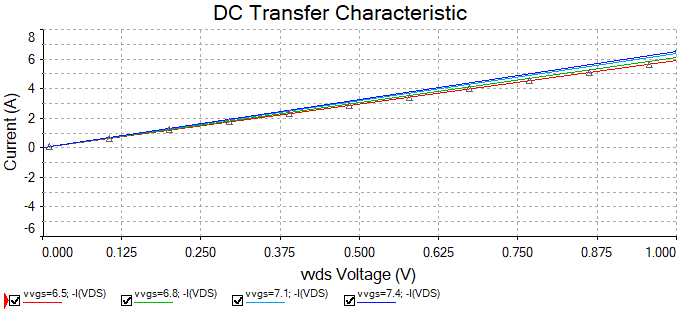
\includegraphics[width=\linewidth,height=5cm]{simul_irfp240} 
	\caption{Resultados de simulación del mosfet IRFP240. En él, se fija $V_{gs}$, y se hace variar $V_{ds}$, y luego se grafica la corriente en función de $V_{ds}$}
	\label{fig:simul_irfp240}
\end{figure}

Los resultados mostrados en la figura \ref{fig:simul_irfp240}, para la corriente que se requiere, los valores de caída de tensión entre Drain y source sobre el mosfet oscilan entre 0.1 Volt y 0.625 Volts (resultado de la simulación). Del grafico (figura \ref{fig:simul_irfp240}) se observa, que una tensión $V_{gs}$ superior a 7 volts, se tiene la misma resistencia aproximadamente, dentro del rango de operación del motor. 


\subsection{Mosfet IRF9530} \label{sub:IRF9530}


Este mosfet es de canal P, y tiene una resistencia $R_{ds}$ máxima de 0.3Ohm. Este mosfet, tiene la conducción de corriente de Source a Drain. La idea de la elección de este componente es igual al anterior. Es decir, se debe elegir una tensión $V_{gs}$ (en este caso negativa), que pueda funcionar sobre todo el rango de operación completo y minimice $V_{ds}$ (también en este caso negativa). El análisis es similar al transistor anterior, y se debe partir por que la $V_{gs}$ mínima es de -4Volts y la máxima soportada entre $V_{gs}$ es de -20Volts. Por este motivo, la tensión debe oscilar entre -20Volts y -4volts(ver \cite{IRF9530}). 
El criterio para seleccionar la tension $V_{gs}$ es reducir lo más posible $V_{ds}$ en todo el rango de operación de la corriente. Las curvas del transistor a 25ºC se muestran a continuación: 

\begin{figure}[ht!] 
	\centering 
	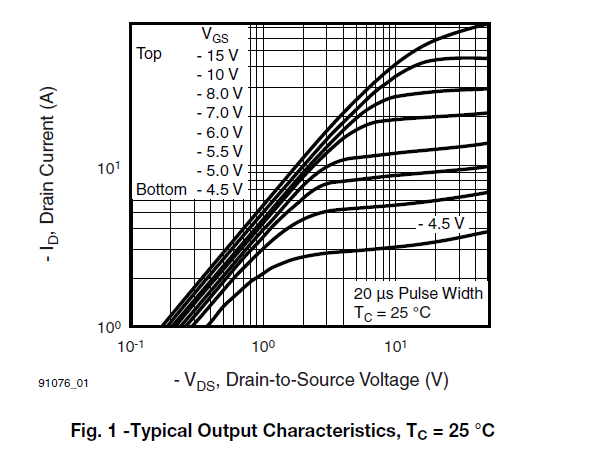
\includegraphics{datasheet_irf9250}
	\caption{Curva $V_{gs}$ frente a $I_{DS}$ del transistor IRFP9530}
\end{figure}

De la curva anterior, se obtiene que se debe reducir la tensión entre gate y source menor a -5.5Volts, siendo el más óptimo -15Volts, que produce una $V_{ds}$ menor en todo el rango de operación. El punto óptimo ocurre con $V_{gs}$ de -15v, pero simplemente, relajando las condiciones, podemos ver que con $V_{gs} <-7Volts$, se encuentra en la misma pendiente.   



\subsection{Transistor BC548} 


Este transistor es de propósito general, tipo NPN, y se va a utilizar para controlar el disparo de los transistores mosfet. En el caso de corte, corriente en la base es nula, y la tensión entre colector y emisor, es la tensión de la fuente $V_{cc}$ en la figura \ref{fig:calc_RB}. Esta tensión, se debe asegurar que sea soportada por el dispositivo para no dañarlo. La máxima tensión soportada entre colector y emisor es de 30Volts (ver \cite{BC548}). También, debe considerarse el otro estado: el estado de saturación. En esta condicion, el fabricante brinda la corriente de colector($I_c$) máxima que es soportada por el dispositivo(esta limitación, se debe a la potencia que debe disipar el dispositivo en estas condiciones) y la tensión $V_{CE}$ en este estado. En estado de corte y saturación deja de valer la relación de ganancia de corriente de colector a corriente de base(\ref{eq:bjt_zona_act}) y en las hojas de datos, este dato aparece con el nombre de $H_{FE}$). La curva característica de este transistor se muestra a continuación( extraída de la hoja de datos).

\begin{figure}[ht!]
	\hspace{-20mm}
	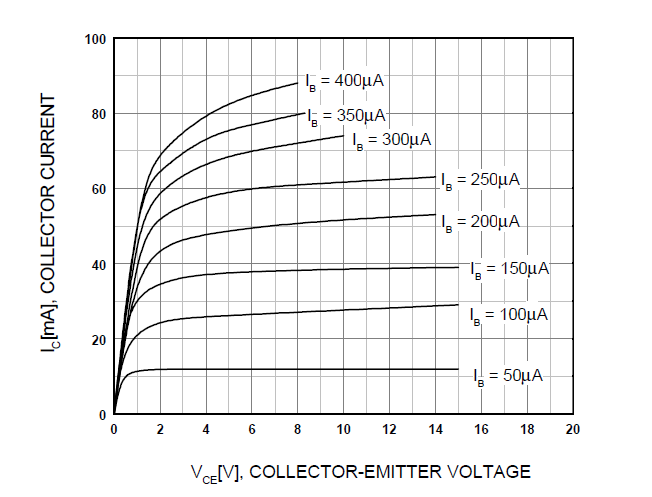
\includegraphics{curvas_bjt_bc548}
	\caption{Diagrama $V_{CE}$ vs $I_c$ del transistor BC548}
\end{figure}


Por tanto, de las especificaciones extraídas del datasheet, en el estado de saturación debe cumplirse lo siguiente: 
\begin{equation*}
	0<V_{CE}\leq0.25 \qquad I_c<100\text{ma} \qquad \frac{I_c}{I_b} = 10
\end{equation*}
Los datos anteriores son válidos si $I_c = 10\text{ma}$ e $I_b = 0.5\text{ma}$
  
En el caso de corte, la corriente por la base es nula, y la tensión entre la base y el emisor es menor a 0.7 Volts, y con esta configuración, se obtiene que la corriente de colector es nula. Por ende, el diseño debe plantearse en términos de la corriente máxima de colector, y que la corriente de diseño sea menor. 

\section{Diseño del puente H – Control de las llaves }

Con los datos que se presentaron en la sección anterior, se va a realizar un primer diseño del puente H, donde solamente con dos transistores BJT se hará el control de las cuatro llaves. El segundo diseño, usa cuatro transistores, donde unimos dos por la base para evitar el cortocircuito. El problema del diseño del puente H es el control de las llaves para evitar el cortocircuito al cargar el código sobre el microcontrolador. Se han realizado pruebas sobre transistores de muy bajo costo, y este problema ha sido notorio, destruyendo varios transistores. Por lo tanto, al utilizar estos mosfet de potencia, al tener un coste elevado, requiere tener precauciones sobre el diseño, a fin de evitar estos cortocircuitos. 

\subsection{Primer diseño – Control de 4 Llaves mediante dos BJT }

El primer diseño, se deben calcular todas las resistencias de control, para poder evitar el cortocircuito. El diseño se muestra a continuación, y luego se muestran los detalles del cálculo de las resistencias

\begin{figure}[ht!]
	\centering
	\includegraphics[scale=0.6]{primer_diseño_h}
	\caption{Primer diseño del puente H. Esta configuración impide el cortocircuito en caso que los transistores mosfet se activen de forma accidental}
	\label{fig:primer_puente_h}
\end{figure}

Donde se deben calcular las resistencias en base a los valores dichos en la sección \ref{sub:bjt_llave}. $V_{g3}$ y $V_{g4}$ deben tener el valor de 7V, y para el análisis circuital, lo suponemos fijo. Las resistencias, se calculan de un único lado, ya que son las mismas del otro lado por simetría del circuito. Además, se debe calcularse la resistencia de base en cada transistor BJT, que no se muestra. Luego del cálculo de todas las resistencias se calculan estas en base a la saturación del transistor. La tensión de alimentación es de 24Volts($V_{cc}$)

Los valores de tensión de $V_{g1}$ y $V_{g2}$ deben ser los mismos, pero deben cumplir dos condiciones, una cuando el transistor Q5(o Q6) este abierto (o cortado), debe tener una tensión menor a aquella que hace conducir el transistor. El $V_{gs}$ de los mosfet de canal P oscila entre -2v y -4volts. Por tanto, $V_{gs1} = V_{s} – V_{g1} = V_{cc} – V_{g1} = 24 -V_{g1}$. Dado  que $V_{gs1}>-2v $, entonces  queda el siguiente resultado analizando ambos extremos: 
\hspace{-10mm}
\begin{align} 
		V_{gs1} &>-2V \rightarrow V_{g1} - V_s>-2V  \rightarrow V_{g1} - V_{cc}>-2V\rightarrow V_{g1}-24V>-2V \rightarrow V_{g1}>22V \label{eq:margen_inf_mos} \\ 
 		V_{gs1} &>-4V \rightarrow V_{g1} - V_S>  -4V \rightarrow V_{g1} - V_{cc}> -4V \rightarrow V_{g1} - 24V>-4V \rightarrow V_{g1}>20V  
%		\label{eq:margen_sup_mosf}
\end{align}
 
Por tanto, cuando los transistores mosfet de canal N conduzcan, debe existir una tensión mayor a 22 volts para un funcionamiento seguro de corte del transistor mosfet de canal P.  
%
Análogamente, cuando el transistor Q5 o Q6 estén conduciendo, el mosfet de canal P debe ponerse en conducción. Para esta situación, se plantea una tensión Vgs que sea menor a -7 volts, se elige $V_{gs}  = -15$, que es lo óptimo según la sección \ref{sub:irfp240}. $V_{gs1} = -15\rightarrow Vg 1= -15+V_{cc} = 24-15 = 9$ Volts. Si esto es posible, entonces se podrá realizar, si no, se deberá recurrir a una $V_{g1}$ mayor, pero deberá ser subóptimo, aceptando algunos milivolts más de pérdida en $V_{ds}$. 
%
Para realizar los cálculos, se empieza suponiendo que el transistor Q5 está conduciendo y Q6 está cortado (figura \ref{fig:primer_puente_h}). En esta condición se debe analizar los siguientes circuitos (se ha utilizado el mismo transistor, ya que el circuito del lado opuesto es el mismo): 
\begin{figure}[ht!]
	\begin{subfigure}{0.45\linewidth}
		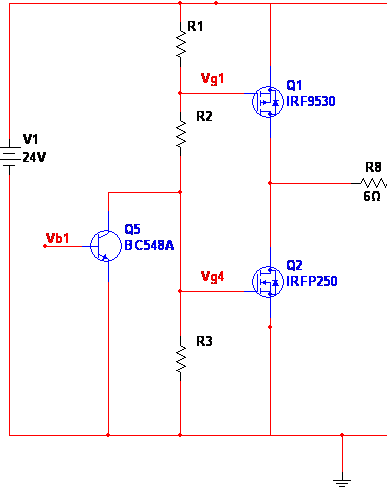
\includegraphics[scale=0.5]{analisis_rama_puente_1}
		\caption{Diagrama de circuito, con el transistor Q5 en estado de corte}
		\label{fig:bjt_cortado}
	\end{subfigure}
\hfill 
	\begin{subfigure}{0.5\linewidth}
	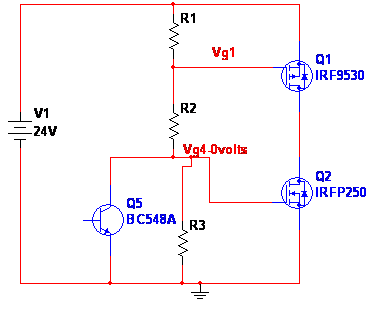
\includegraphics[height=6cm]{analisis_rama2_puente_1}
		\caption{diagrama del circuito a analizar con el transistor Q5 en estado de conducción. Se observa, que $V_{g4}$ }
		\label{fig:q_cortado}
	\end{subfigure}c
\caption{Esquema de los transistores de control del puente H}
\end{figure}

Del circuito, se observa que la resistencia crítica para calcular es $R_{1}$(o $R_{4}$). Esta resistencia, debe cumplir que permita la apertura y cierre del mosfet en base a la tensión que este aplicada sobre ella. Por tanto, se empieza calculando esta resistencia, y luego se calculan las demás. 
En el caso de que Q5 esté en estado de corte(ver figura \ref{fig:q_cortado}) se debe cumplir que $V_{g}>22V $(ver ecuación \ref{eq:margen_inf_mos}). 
  
Se  denomina a la corriente que circula por el circuito de la figura \ref{fig:q_cortado}, $I_c$ y a la corriente que circula por el circuito de la figura \ref{fig:bjt_cortado}, $I_S$ (esta corriente circula por $R_1$,$R_2$ y $R_3$). Como $Vg>22V$,se analiza el circuito de la figura \ref{fig:bjt_cortado} quedando la siguiente desigualdad: 
\begin{equation}\label{eq:isat}
	V_{g1} = V_{cc} - I_cR_1>22V \xrightarrow{V_{cc} = 24 } I_cR_1<2V
\end{equation}

Para el caso de la saturación (figura \ref{fig:q_cortado}), se plantea que la tensión $V_{gs}<-15Volts$. Con esto se obtiene una segunda desigualdad($V_{gs}=V_{g1} - V_{cc}$):

\begin{equation}
	V_{g1} - V_{cc} <-15V \xrightarrow{ V_{cc}=24}V_{g1}<9V  
\end{equation}

Luego, con la ecuación anterior, se calcula cual debe ser el valor para $I_s$, realizando el análisis circuital de la figura \ref{fig:q_cortado}, se tiene la siguiente ecuación usando leyes de Kirchhoff: 
\begin{equation}
	V_{g1} = V_{cc} - I_sR_1<9V\xrightarrow{V_{cc}=24V} I_SR_1>15V
\end{equation}

Luego, de la desigualdad anterior, se propone $I_s=1$ma, con esto, la desigualdad anterior, da por resultado una resistencia $R_1>15$K$\Omega$. Se elige una $R_1=16$K$\Omega$, luego se calcula la resistencia total, con esta corriente, siendo la resistencia total en saturación viene dada por $R_t = R_1+R_2$. La resistencia total($R_t$) y la resistencia $R_2$ viene dada por: 
\begin{equation}
	R_t = \frac{V_{cc}}{1\text{ma}} =\frac{24}{1\text{ma}} = 24K\Omega\xrightarrow{R_t = R_1+R_2} R_2 = 24K\Omega - 16 K\Omega = 9K\Omega   
\end{equation}

Luego, resta analizar el estado de saturación del transistor Q5(o Q6). Con la ecuación \ref{eq:isat}, se calcula el valor de $I_s$ con el valor de $R_1 = 16k\Omega$. Con esto, el valor $I_c<\frac{2V}{16k\Omega}=0.125$ma. Se selecciona el valor de $I_s=0.1$ma, y se calcula el valor de la resistencia $R_3$ 

Para que exista el valor propuesto de $I_c$, se debe plantear que la resistencia total en este estado, viene dada por $R_t=R_1+R_2+R_3 = \frac{24V}{I_s}$, de esta expresión resulta $R_3 = 216K\Omega$

Luego, se debe verificar si cumplen las condiciones de corte y saturación de los transistores mosfet con estas resistencias. Si se realiza el análisis con las resitencias calculadas, resulta en la siguiente tabla: 
\begin{table}[ht!]
\centering
\begin{tabular}{|c|c|c|}
	\hline 
	 & corte & saturación \\ \hline 
	 $V_{g1}$ &22.5V & 21.89 \\ \hline 
	 $V_{g4}$ &6.96V & x \\ \hline 
\end{tabular}
\caption{Tabla resumen de la primera iteración.}
\end{table} 

Luego se realiza el mismo procedimiento, donde se cambia la $I_s$ inicial. La siguiente tabla, resume todas las iteraciones realizadas. 

% primera iteracion -----------
\begin{table}[h]
%	\hspace{-30mm}
\resizebox{\linewidth}{!}
{
 \begin{threeparttable}
	\begin{tabular}{|c|c|c|c|c|c|c|c|c|c|c|c|} 
%--- fila con titulos de tabla  -----------------------% 
		 \hline
		 \multicolumn{5}{|c|}{ \multirow{2}{20mm}{parámetros circuitales}} & 
		 \multicolumn{3}{c|}{estado} & 
		 \multicolumn{2}{c|}{\multirow{2}{20mm}{Condiciones de corte}} & 
		 \multirow{2}{20mm}{Condiciones de sat} 
		 & \multirow{3}{20mm}{cumple req} \\ \cline{6-8}
%---- segunda fila ---- 
		 \multicolumn{5}{|c|}{} &  \multicolumn{2}{c|}{corte} & saturación & \multicolumn{2}{c|}{} && \\ \cline{1-11}
% -----------------------variables -----------------------%		 
		 $I_s$[ma]&$R_1$[K$\Omega$]&$R_2$[K$\Omega$]&$I_c$[ma]&$R_3$[K$\Omega$] & $V_{g1}$[V]& $V_{g4}$[V]& $V_{g1}$[V] & $V_{g1}>22V$ & $V_{g4}>7v$ & $V_{g1}<9V$ & \\ \hline 
%----------------- datos ----------------------------------% 
	1 & 16&9&0.1 &216&22.5 &6.96 &21.89 &\checkmark & \xmark  & \xmark & no \\ \hline
	2 & 8 & 4 & 0.2 & 108 & 22.4 & 21.6 & 16 & \checkmark & \checkmark & \xmark & no \\ \hline   	
	5 & 3.1 & 1.7 & 0.5 & 43.2 & 22.45 & 21.6 & 8.5 & \checkmark & \checkmark	& \checkmark &Sí\tnote{1} \\ \hline 
	3 & 6 & 2 & 0.3 & 72 & 22.2 & 21.6 & 6 & \checkmark & \checkmark & \checkmark & si\tnote{1}   \\ \hline
	10 & 2 & 0.4 & 0.8 & 27.6 & 22.4 & 22.08 & 4 & \checkmark & \checkmark & \checkmark & si \tnote{1} \\ \hline 
	\end{tabular}
	\begin{tablenotes}
		\small
		\item[1] En este caso, se cumplen las condiciones para su uso, solo que el transistor mosfet elegido soporta una tension máxima de 20 volts entre Gate y Source. 
	\end{tablenotes}
	\end{threeparttable}
}
\caption{Valores que se obtienen mediante el proceso de iteración}
\end{table}	

La tabla anterior,se ovserva que las unicas posibilidades posibles son con $I_s$de 3ma,5ma o 10 ma. Estos valores, si bien cumplen, son destructivos para el transistor de canal N, pues su tensión máxima soportada entre gate y source es 20V. De la tabla, se analiza que al aumentar la corriente de saturación, los valores de tensión, permanecen casi sin cambio a partir de 3ma. Por este motivo, se han relajado las condiciones para los mosfet, para que trabajen en un punto subóptimo de trabajo. El procedimiento es el mismo, pero cambiando sus valores de requerimientos para la tensión entre Gate y Source. La siguiente tabla, arroja los resultados: 



% segunda iteracion -----------
\begin{table}[h]
	%	\hspace{-30mm}
	\resizebox{\linewidth}{!}
	{
		\begin{threeparttable}
			\begin{tabular}{|c|c|c|c|c|c|c|c|c|c|c|c|} 
				%--- fila con titulos de tabla  -----------------------% 
				\hline
				\multicolumn{5}{|c|}{ \multirow{2}{20mm}{parámetros circuitales}} & 
				\multicolumn{3}{c|}{estado} & 
				\multicolumn{2}{c|}{\multirow{2}{20mm}{Condiciones de corte}} & 
				\multirow{2}{20mm}{Condiciones de saturación} 
				& \multirow{3}{20mm}{cumple req} \\ %\cline{6-8}
				%---- segunda fila ---- 
				\multicolumn{5}{|c|}{} &  \multicolumn{2}{c|}{corte} & saturación & \multicolumn{2}{c|}{} && \\ \cline{1-11}
				% -----------------------variables -----------------------%		 
				$I_s$[ma]&$R_1$[K$\Omega$]&$R_2$[K$\Omega$]&$I_c$[ma]&$R_3$[K$\Omega$] & $V_{g1}$[V]& $V_{g4}$[V]& $V_{g1}$[V] & $V_{g1}>22V$ & $V_{g4}>7v$ & $V_{g1}<17V$ & \\ \hline 
				%----------------- datos ----------------------------------% 
				2 & 10 & 2 & 0.1 &228 &23 &22.8 & 4 &\checkmark &\checkmark &\checkmark &Sí\tnote{1} \\ \hline 
				1 & 8 & 16 & 0.1 &216 &23.2 &21.6 & 16 &\checkmark &\checkmark &\checkmark &Sí\tnote{1} \\ \hline 
				5 & 2.4 & 2.4 & 0.5 &43.2 &22.8 &21.6 & 12 &\checkmark &\checkmark &\checkmark &Sí\tnote{1} \\ \hline 
				
				10 & 1.3 & 1.1 & 1 &21.6 &22.7 &21.6 & 13 &\checkmark &\checkmark &\checkmark &Sí\tnote{1} \\ \hline 			
	\end{tabular}
	\begin{tablenotes}
	\small
	\item[1] En este caso, se cumplen las condiciones para poder usarlo, solo que la limitante es el dispositivo mosfet elegido, ya que su tensión máxima que soporta entre Gate y Source es 20 volts. 
	\end{tablenotes}
	\end{threeparttable}
}
\caption{Valores que se obtienen mediante el proceso de iteración}
\end{table}	

Lo que se observa en ambas iteraciones, que hay una relación de compromiso al seleccionar $R_1$, y al cambiar esta elección, influye sobre $R_3$, y genera que la tensión entre Gate y source del mosfet de canal P, esté al límite, mientras la tensión entre gate y source del mosfet de canal N es superior a la permitida. Observando las iteraciones, se concluye, que, de forma casi independiente a la elección de las resistencias, las tensiones caídas son aproximadamente las mismas. No se puede garantizar la no conducción con estos valores de resistencias, pero se garantiza la destrucción del mosfet de canal N, al superar su máxima tensión de gate y source. Este hecho, motiva el rediseño del control de los transistores mosfet. 


\subsection{Segundo Diseño – Control de 4 Llaves mediante cuatro BJT}


Al ser casi independiente el circuito con el valor de las resistencias, debe rediseñarse, aumentando la tensión, en caso del canal P, y disminuirla, en caso del canal N. Se ha rediseñado el control de los transistores mosfet, usando 4 transistores BJT que   trabajen en contrafase. El circuito rediseñado es el siguiente: 
\begin{figure}[ht!]
	\centering
	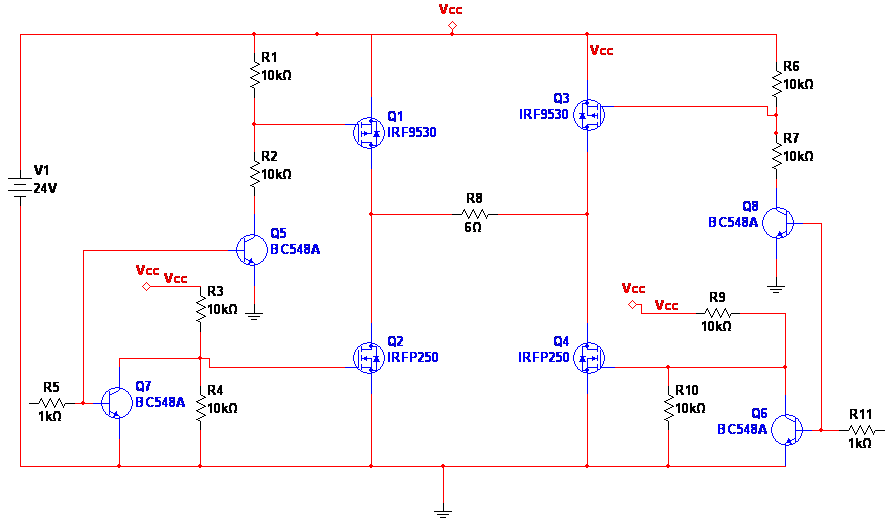
\includegraphics[scale=0.5]{segundo_puente_h} 
	\caption{Rediseño del circuito para evitar el cortocircuito entre los mosfet} 
	\label{fig:segundo_puente_h}
\end{figure} 
Este circuito, si se ponen todas las resistencias del mismo valor, cumple con todos los requisitos, pues la tensión, es la mitad, y no permite la destrucción del mismo. Si se consideran, los casos de tolerancia de las resistencias, ocurre lo mismo, suponiendo una tolerancia del 10\%, la mitad de la tensión subirá 10\% o disminuirá 10\% (caso extremo), la tensión en los terminales entre gate y source es de $12 \pm 1.2$, que está dentro de los rangos de operación. En este caso, la figura muestra de 1K$\Omega$, pero se pondrán todas resistencias de 10K$\Omega$. 

Si observamos las llaves, considerando como entrada a las resistencias R11 y R5,como entradas digitales, se observa el siguiente comportamiento sobre los transistores

\begin{table}[ht!]
	\centering
	\hspace{-10mm}
	\begin{tabular}{|p{2cm}|p{2cm}|p{2cm}|p{2cm}|p{2cm}|p{2cm}|p{2cm}|}
		\hline
		Estado entrada $R_5$ & Estado entrada $R_11$& Estado Q5 & Estado Q6&Estado Q7&Estado Q8&Mosfet Activados \\ \hline   
		0 & 0&corte &corte &corte &corte &Q2 y Q4 \\ \hline 
		1&0&saturación&saturación& corte& corte &Q1 y Q4 \\ \hline
		0& 1& Corte& Corte &Saturación& Saturación &Q2 y Q3 \\ \hline
		1 &1 &Saturación &Saturación& Saturación& Saturación& Q1 Y Q3 \\ \hline
	\end{tabular}
\end{table}

Se observa en la tabla anterior, que no existe ningún caso en el cual se genere el cortocircuito. La tabla anterior, se obtiene realizando el análisis circuital sobre los controles de
las llaves, mostrados en la figura \ref{fig:segundo_puente_h}. 

Para el cálculo de $R_5$, se debe suponer el transistor Q5 y Q7, o los complementarios del lado derecho de la figura \ref{fig:segundo_puente_h}, en estado de saturación. En este estado, la resistencia de colector para el transistor Q5(o Q8) es de $R_{TCQ5}=20K\Omega$ y para el otro transistor(Q7 o Q6) es de $R_{TCQ7}=20K\Omega$. Con estos valores, se calcula la $I_{CQ5SAT}$ e
$I_{CQ7SAT}$(ver ecuación \ref{eq:IC_sat}). 

\begin{equation}
	\begin{cases}
		I_{CQ5SAT} = \frac{V_{CC}-V_{CEsat}}{R_{TCQ5}}\xrightarrow{V_{CC}>>V_{CEsat} y V_{CC}=24V }I_{CQ5SAT} = \frac{24V}{20K\Omega} = 1.2\text{ma} \\ 			
		I_{CQ7SAT} = \frac{V_{CC}-V_{CEsat}}{R_{TCQ7}}\xrightarrow{V_{CC}>>V_{CEsat} y V_{CC}=24V }I_{CQ7SAT} = \frac{24V}{10K\Omega} = 2.4\text{ma}  	
	\end{cases}
\end{equation}

La corriente de base mínima para cada transistor, se basa en en el peor caso de la ganancia $H_{FE}$, en el caso del transistor BC548, el peor caso ocurre cuando $H_{FE} = 200$(ver \cite{BC548}). Con estos valores, se obtienen las corrientes mínimas por la base de cada transistor(ver ecuación \ref{eq:IB_min}): 
\begin{equation}
	\begin{cases}
		I_{bQ5min} = \frac{I_{CQ5SAT}}{H_{FEmin}} = \frac{1.2\text{ma}}{200} = 6\mu A  \\
		I_{bQ5min} = \frac{I_{CQ5SAT}}{H_{FEmin}} = \frac{2.4\text{ma}}{200} = 12\mu A 
	\end{cases}
\end{equation}
Por este motivo, la corriente que se requiere para la resistencia $R_5$ debe ser mayor a la suma de ambas corrientes, para garantizar la saturación. La corriente $I_{bminR_5} = 12\mu A + 6\mu A = 18\mu A $ y se utiliza la ecuación \ref{eq:select_rb}, para calcular los posibles valores de $R_5$. Se realiza este calculo(usando $V_{p}=5V$ que es la tensión del puerto de salida del microcontrolador, y $V_{BE}=0.6V$), da por resultado $R_5<244K\Omega$. Se selecciona $R_5=1K\Omega$. 

Luego, se realiza una simulación, donde en la resistencia $R_5$ y $R_{11}$ se coloca a contrafase una onda cuadrada de 500Hz de periodo. Se coloca un osciloscopio entre las terminales de $R_8$, en la simulación. El resultado, se observa a continuación: 
\begin{figure}[ht]
	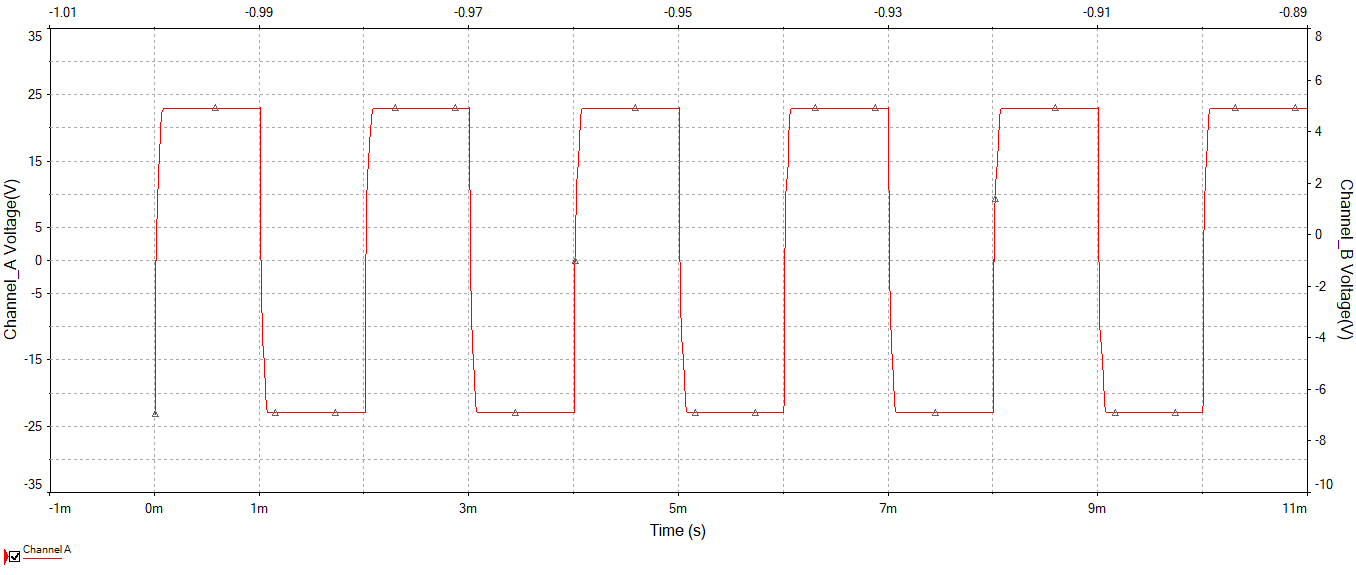
\includegraphics[scale=0.5]{simulacion_puente_2}
	\caption{Simulación del circuito de la figura \ref{fig:segundo_puente_h}}
\end{figure}

Se observa, que la tensión cambia de sentido, como se esperaba. Esta carga que se ha puesto, es para probar el puente H. En futuros desarrollos, se espera poder tener un modelo completo del motor, para poder realizar la simulación, y el control de manera adecuada (control por PID). 

\section{Modelado térmico y Selección del disipador} 


Dado que por los transistores mosfet, circulará una corriente de 7 ampere aproximadamente, este tiene que evacuar el calor de su interior hacia el ambiente por alguno de los medios conocidos para disipación de calor(convección, radiación y conducción) Esta cantidad de corriente, hace que el transistor mosfet, eleve su temperatura, haciendo necesario algún medio para evacuar el calor hacia el exterior. El dispositivo utilizado para extraer el calor y enviarlo al ambiente, se conoce con el nombre de disipador.  Este dispositivo es el encargado de evacuar el calor del interior del dispositivo hacia el medio ambiente que lo rodea(en realidad, le brinda un mecanismo de evacuación del calor).

El proceso de análisis de la temperatura en el dispositivo, y y en el disipador, es excesivamente complejo, se toma un modelo eléctrico equivalente. En este modelo se considera una ``resistencia térmica'', una potencia disipada, y una diferencia de potencial, representada por una diferencia de tensión. 

La resistencia térmica, podemos verla del siguiente modo: si tenemos una barra de algún material conductor del calor, y la diferencia de temperaturas en ambos extremos es diferente, existe un flujo de calor, de aquella que está a mayor temperatura hacia aquella que está a temperatura menor. Por lo tanto, al existir un flujo de energía de un extremo a otro, podemos plantear que existe una potencia térmica (energía por unidad de tiempo). Esta potencia se define por: 
\[
	P_{cond} = \frac{\lambda A \Delta T}{d}
\]
Siendo 
\begin{flalign*}
	&\lambda:\text{conductividad térmica del material} &  \\
	&A : \text{Área de sección transversal} & \\
	&\Delta T \text{diferencia de temperaturas}& \\
	&d:\text{distancia entre ambas caras} & 
\end{flalign*}

Se nota, de la expresión anterior, que se puede relacionar con una resistencia térmica, denotada como $R_{\theta cond} $, definida por: 

\begin{equation} \label{eq:calc_res_term}
	R_{\theta cond} = \frac{\Delta T}{P_{cond}} = \frac{\lambda A}{d}
\end{equation}

Si el calor, debe fluir, a través de varios materiales, entonces se plantea diferentes resistencias en serie, siendo la resistencia térmica total del sistema, es la suma de todas las resistencias. Por tanto, la diferencia de temperaturas, es igual a la potencia por la resistencia total. Esto es análogo a un circuito eléctrico, donde la corriente es la potencia, las resistencias son la resistencia térmica, y la diferencia de tensión, es el producto de la potencia por la resistencia. La siguiente imagen aclara este concepto:

\begin{figure}[ht!]
	\centering
	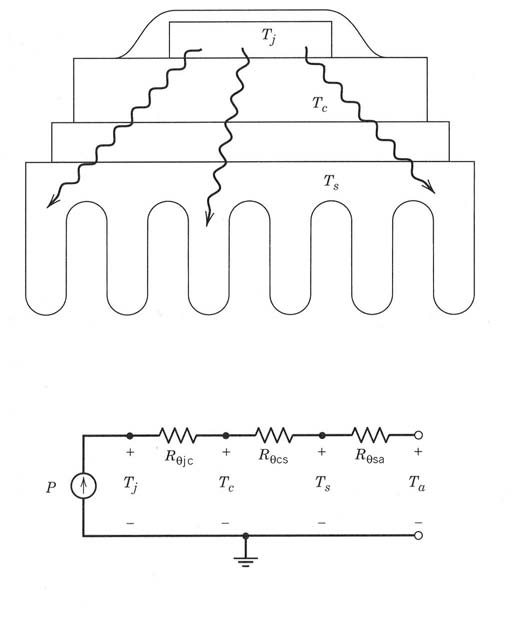
\includegraphics[scale=0.4]{modelo_termico_general}
	\caption{Relación entre potencia térmica y eléctrica para el cálculo de disipadores. Además, se muestran el camino seguidos por el calor en un dispositivo electrónico que posea disipador, y el modelo térmico en la parte de debajo de la figura principal}
	\label{fig:modelo_termico_disip}
\end{figure}

Luego, se debe ser capaz de decidir sobre la elección del disipador. Este modelo térmico eléctrico es el que se va a utilizar para elegir el disipador. El mecanismo explicado hasta aquí, es el mecanismo de conducción. Se tiene otro mecanismo que es importante, es el de radiación. Este mecanismo, permite la disipación de calor, en base al área que este en contacto con la otra superficie. En nuestro caso, el disipador, está en contacto con el medio ambiente. El tercer mecanismo de evacuación del calor, carece de interés en este trabajo.

\subsection{Selección del disipador} 

El disipador es el elemento que extrae el calor desde dentro del dispositivo hacia el medio ambiente. Por tal motivo, se debe elegir un disipador que cumpla con las condiciones de diseño. Es responsabilidad del diseñador, mantener la temperatura dentro del dispositivo, dentro de límites razonables, para el buen funcionamiento del dispositivo, y evitar su destrucción por temperatura. 

La selección del disipador, depende de la máxima temperatura de juntura admisible por el dispositivo. Teniendo, la TJ,MAX, la temperatura ambiente máxima TA,MAX, la máxima tensión de operación, y los puntos de operación del dispositivo, y las perdidas por conmutación (promediando la energía en un periodo de conmutación),la máxima resistencia que este dispositivo posee. Por lo tanto, se estima que la potencia de pérdida, es la potencia en estado activo más la potencia perdida por conmutación. Si usamos estos datos, obtenemos la resistencia máxima entre temperatura y ambiente: 
\begin{equation*}
	R_{\theta JA} = \frac{T_{jmax}- T_{jmin}}{P_{cond}}
\end{equation*}

Esta resistencia, se obtiene de las hojas de datos de los dispositivos, y la resistencia entre la carcasa y el ambiente, es un dato del fabricante del disipador. 

En caso que el fabricante, nos brinde la resistencia entre la juntura y la carcasa, entonces, se debemos calcular la resistencia entre el disipador y el ambiente. Luego, seleccionamos un disipador con menor resistencia a la encontrada. 

\subsection{Datos de transistores mosfet - cálculo de resistencia térmica }

Primero explicará cómo realizar el cálculo sobre el mosfet de canal P, y el de canal N, es análogo, y simplemente se darán los resultados. 

El transistor IRFP9530, es un transistor MOSFET tipo P, que tiene una temperatura de juntura máxima de 175º C. De la hoja de datos(ver \cite{IRF9530}),se extraen los siguientes parámetros dados por el fabricante: 
\begin{table}[ht!]
	\centering
	\begin{tabular}{|c|c|c|c|c|}
		\hline 
		\multicolumn{5}{|c|}{parámetros térmicos transistor IRFP9530}\\ \hline 
		Parámetro & Simbolo & tipico & máximo & unidad \\ \hline 
		Máxima juntura - Ambiente &$R_{\theta JA}$ & - &62 & \multirow{3}{*}{ºC/W} \\ \cline{1-4} 
		Juntura carcasa con Grasa siliconada &$R_{\theta CS}$ & 0.5 &-& \\ \cline{1-4} 
		Máxima juntura carcasa(Drain) &$R_{\theta JC}$ & - &1.7& \\ \hline
	\end{tabular}
\caption{Tabla resumen de los parámetros térmicos del transistor IRFP9530(extraidos de \cite{IRF9530})} 
\label{tab:par_ter_irfp9530}
\end{table}


Se observa en la tabla anterior, que la máxima resistencia entre la juntura y el ambiente es de 62ºC/W. Si se coloca un disipador, como en nuestro caso, obtenemos una resistencia de 0.5ºC/W, la  máxima resistencia juntura ambiente es de 1.7ºC/W

Para determinar si el uso del disipador es necesario, se plantea el siguiente circuito térmico: 
\begin{SCfigure}[50][h]
\vspace{-20mm}	
\caption{Diagrama del circuito térmico sin disipador}	
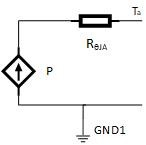
\includegraphics{circuito_termico_1}

\end{SCfigure}
\newline 








Donde para calcular los valores, usamos $R_{\theta JA}= 62^\circ C/W$ y la temperatura ambiente, la suponemos 50º C. Esto es por dos motivos, el primero es que, en verano, el sol puede darle de frente, el otro, es que, al estar montado sobre una estructura de metal, que está expuesta directamente al sol, va a ser capaz de transferir su calor. La potencia disipada por el mosfet (corriente máxima 5ampere) en este caso es: 
\[
	P = (7A)^2 \times 0.3 V = 14.7 W 
\]

Por esto, la temperatura de juntura tiene por resultado: 
\begin{equation} \label{eq:temp_juntura}
T_j  = P R_{\theta JA}+T_a  = 515^\circ C 
\end{equation}

Esta temperatura de juntura es destructiva para el transistor. Por este motivo, debe ponerse un disipador. 

Si el circuito requiere un disipador, además de él, agregamos una capa aislante, grasa siliconada y el mismo disipador. Este modelo térmico se muestra a continuación:

\begin{figure}[ht!]
	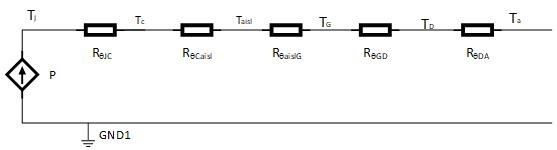
\includegraphics{circuito_termico_2}
	\caption{Modelo térmico completo para el cálculo de la resistencia térmica de un disipador}
	\label{fig:circuito_termico_calc_disip}
\end{figure}

Donde las resistencias son las siguientes: 
\begin{itemize}
	\item ${R_\theta JC} $:resistencia entre la juntura y la carcasa del dispositivo: en este caso es de 1.7 ºC/W  
    \item ${R_\theta Caisl}$: resistencia térmica entre la carcasa y el aislante
    \item ${R_\theta aislG}$: resistencia térmica entre aislante y la grasa siliconada
	\item ${R_\theta GD}$: resistencia térmica entre la grasa y el disipador
	\item ${R_\theta DA}$: resistencia térmica del disipador
\end{itemize}

De la figura \ref{fig:modelo_termico_disip},se observa que se tienela suma de las tres resistencias :$ R_{Caisl}+ R_{aislG}+ R_{GD} = 0.5ºC/W$(valor mínimo, según la tabla \ref{tab:par_ter_irfp9530}). Estos datos se usan para realizar el cálculo del disipador. En realidad, se deben obtener estos valores de resistencias térmicas de forma experimental o mediante hojas de datos.
 
Para el cálculo de la resistencia del disipador, se debe hacer que el transistor trabaje a una temperatura de juntura menor a 175ºC, se propone que trabaje a 100º C. Si se observa el circuito de la figura \ref{fig:circuito_termico_calc_disip}, y se realiza el análisis de mallas, obtenemos la $R_{\theta DA}$ mediante la siguiente expresión:
\begin{align} 
R_{\theta dap}& = \frac{\Delta T}{P} - ( R_{\theta JC}+ R_{\theta Caisl} + R_{\theta aislG} + R_{\theta GD}) \frac{100^\circ C - 50^\circ C }{14.7 W} - (1.7^\circ C/ W + 0.5^\circ C/ W ) = 1.2^\circ C/W \nonumber	\\
R_{\theta dap} &=  1.2^\circ C W \label{eq:val:r_term}
\end{align} 

El disipador, debe tener esta resistencia térmica o menor a esta. Cabe destacar, que esta sobredimensionado en corriente, para considearar casos en que existan trabas mecánicas sobre el motor, y que no se dañen los transistores. 

En el caso del mosfet de canal N, se tienen los siguientes parámetros:


\begin{table}[ht!]
	\centering
	\begin{tabular}{|c|c|c|c|c|}
		\hline 
		\multicolumn{5}{|c|}{parámetros térmicos transistor IRFP9530}\\ \hline 
		Parámetro & Simbolo & tipico & máximo & unidad \\ \hline 
		Máxima juntura - Ambiente &$R_{\theta JA}$ & - &40 & \multirow{3}{*}{ºC/W} \\ \cline{1-4} 
		Juntura carcasa con Grasa siliconada &$R_{\theta CS}$ & 0.24 &-& \\ \cline{1-4} 
		Máxima juntura carcasa(Drain) &$R_{\theta JC}$ & - &0.8& \\ \hline
	\end{tabular}
	\caption{Parámetros térmicos del transistor IRFP240N.(extraidos de \cite{IRFP240})} 
	\label{tab:par_ter_irfp240}
\end{table}


En este caso, la potencia disipada por él es menor, ya que su $R_{dsmax}$ es de 0.18$\Omega$ Por lo tanto, su potencia máxima será de 8.82watts, con lo cual, si realizamos el mismo cálculo con la expresión \ref{eq:temp_juntura}, su temperatura de juntura es de 230ºC (su temperatura de juntura máxima es de 150ºC). Por lo tanto, requiere de disipador (se usó la misma temperatura ambiente que para el mosfet de canal P)

Dado, que requiere disipador, se realiza el mismo circuito que la figura \ref{fig:circuito_termico_calc_disip}, pero con la potencia de 8.82 W, y con los valores de la tabla \ref{tab:par_ter_irfp240}, se obtienen los valores de resistencia térmica para el cálculo del disipador: 

\begin{align} 
	R_{\theta dap}& = \frac{\Delta T}{P} - ( R_{\theta JC}+ R_{\theta Caisl} + R_{\theta aislG} + R_{\theta GD}) \frac{100^\circ C - 50^\circ C }{8.82 W} - (0.24^\circ C/ W + 0.83^\circ C/ W ) = 1.2^\circ C/W \nonumber	\\
	R_{\theta dap} &=  4.6^\circ C W \label{eq:val:r_term}
\end{align} 

Por lo tanto, la resistencia térmica del disipador de canal N, debe ser menor a 4.6 ºC/W. Se calculan por separado, ya que no necesariamente los transistores mosfet de canal N y P, estarán montados sobre el mismo disipador.  


\subsection{Ensayos sobre disipadores – Calculo de resistencias térmicas}

Dado el alto coste de los disipadores, y la falta de disponibilidad en el mercado local, lo que se realiza es un ensayo de tipo experimental, donde se miden las resistencias térmicas de  disipadores disponibles para su uso en la institución. Esta medición se realiza sobre el circuito integrado LM7809, que es un regulador de tensión. Se usa este componente debido a su bajo coste y alta disponibilidad en el mercado local. La fuente utilizada, es una fuente de 24V, 10A. Para el ensayo se realiza el siguiente circuito:

\begin{figure}[ht!]
	\centering
	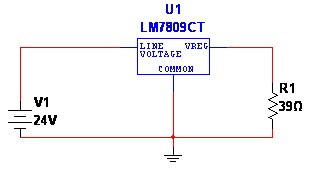
\includegraphics{circuito_prueba_disip}
	\caption{Circuito para realizar el ensayo de los disipadores}
	\label{fig:circ_ensayo_disip}
\end{figure}

La corriente medida por el amperímetro fue de 0.22Ampere. La misma, para calcular la potencia, se realiza el siguiente calculo:
\[
P = 0.22*(24-9)=3.3W
\]

Se toma la medición de la temperatura del ambiente, mediante un sensor DHT11, conectado a un Arduino, y se lo muestra en pantalla, mediante el puerto Serial. La temperatura del disipador, será tomada desde una termocupla adosada a un tester modelo sinometer m890G.

El ensayo consiste en esperar que el disipador alcance una temperatura en estado estable, y se pueda estimar la resistencia térmica mediante la expresión \ref{eq:calc_res_term}, donde la potencia disipada es de 3.3W. La diferencia de temperatura viene dada por la diferencia entre la medida por la  termocupla del tester, con la del ambiente, medida por el sensor DHT11. 

A continuación, se deja una imagen del montaje hecho para medir la temperatura de un disipador. 

\begin{figure}[ht!]
	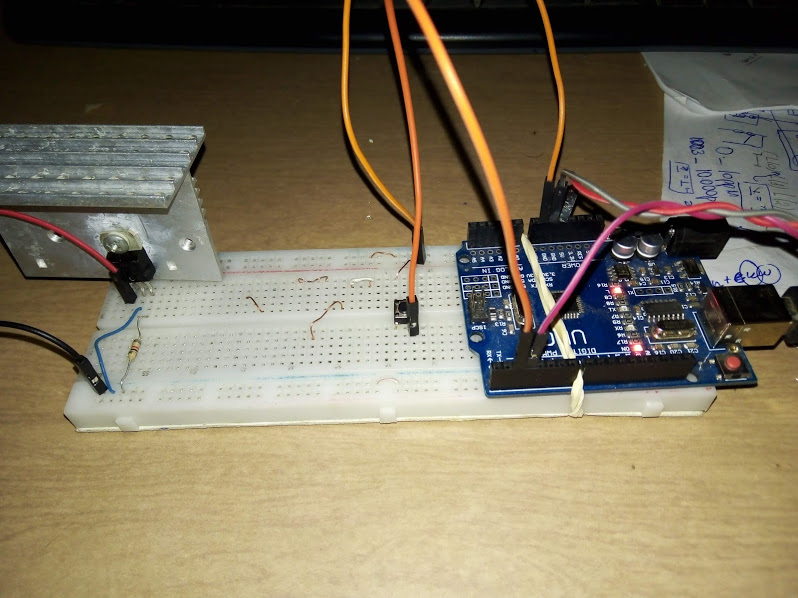
\includegraphics[scale=0.5]{prueba_disipadores_lm}
	\caption{Armado del banco de prueba para medir la resistencia térmica de los disipadores}
\end{figure}

Los disipadores que se miden son los que se muestran en la siguiente imagen: 

\begin{figure}[ht!]
	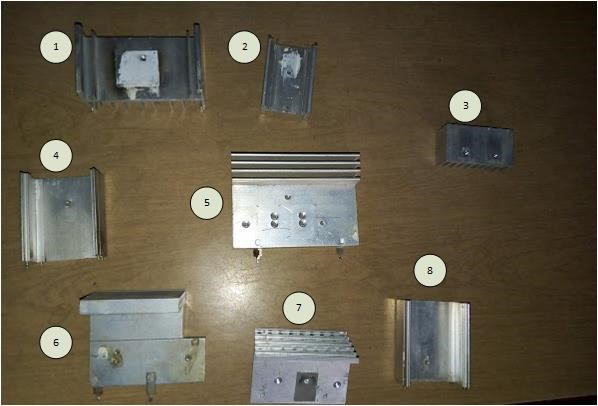
\includegraphics{disipadores_a_ensayar}
	\caption{los disipadores a ensayar. Los mismos se ensayan con el circuito de la figura \ref{fig:circ_ensayo_disip}}
	\label{fig:img_disip_num}
\end{figure}


El circuito térmico, está representado por la figura \ref{fig:circuito_termico_calc_disip}, donde suponemos las resistencias de contacto entre el integrado y el disipador despreciable frente a la resistencia que se desea medir. La resistencia térmica entre la juntura y la carcasa del disipador es de 5°C/W (extraído de la hoja de datos del circuito integrado LM7809). Por tanto, se resuelve el circuito térmico (figura \ref{fig:circuito_termico_calc_disip}) y se desprecia la resistencia de contacto entre el aislante, y grasa disipadora viene dada por la siguiente expresión: 
\begin{equation}
	R_{\theta da} = \frac{T_{disipador}- T_{ambiente} }{P}
\end{equation}
donde P = 3.3W. Los resultados del ensayo se resumen en la siguiente tabla: 
\begin{table}[ht!]
	\centering
	\begin{tabular}{|p{3cm}|c|c|c|}
		\hline  
		Número de disipador(figura \ref{fig:img_disip_num}) & Temperatura final[ºC] & Temperatura ambiente[ºC] & resistencia térmica [ºC/W] \\ \hline 
		 1& 45& 27 &5.45 \\ \hline 
		 2& 53& 22 &9.39 \\ \hline 
		 3& 46& 26 &6.06 \\ \hline 
		 4& 56& 22 &10.3 \\ \hline 
		 5& 45& 22 &6.96 \\ \hline 
		 6& 52& 23 &8.78 \\ \hline 
		 7& 62& 23 &11.8 \\ \hline 
		 8& 45& 22 &13.6 \\ \hline 
	\end{tabular}
\caption{tabla con resultados del ensayo sobre los disipadores de la figura \ref{fig:img_disip_num}}
\end{table}

De la tabla anterior, se observa, que ninguno de los disipadores puede usarse en el armado del puente H.  

El disipador disponible dentro de la institución para su uso, esta sobredimensionado, y este es el que se utilizará, ya que es el único disponible para su utilización. A continuación se deja una imagen del disipador sobre el cual se van a montar los transistores mosfet: 

\begin{figure}[ht!]
	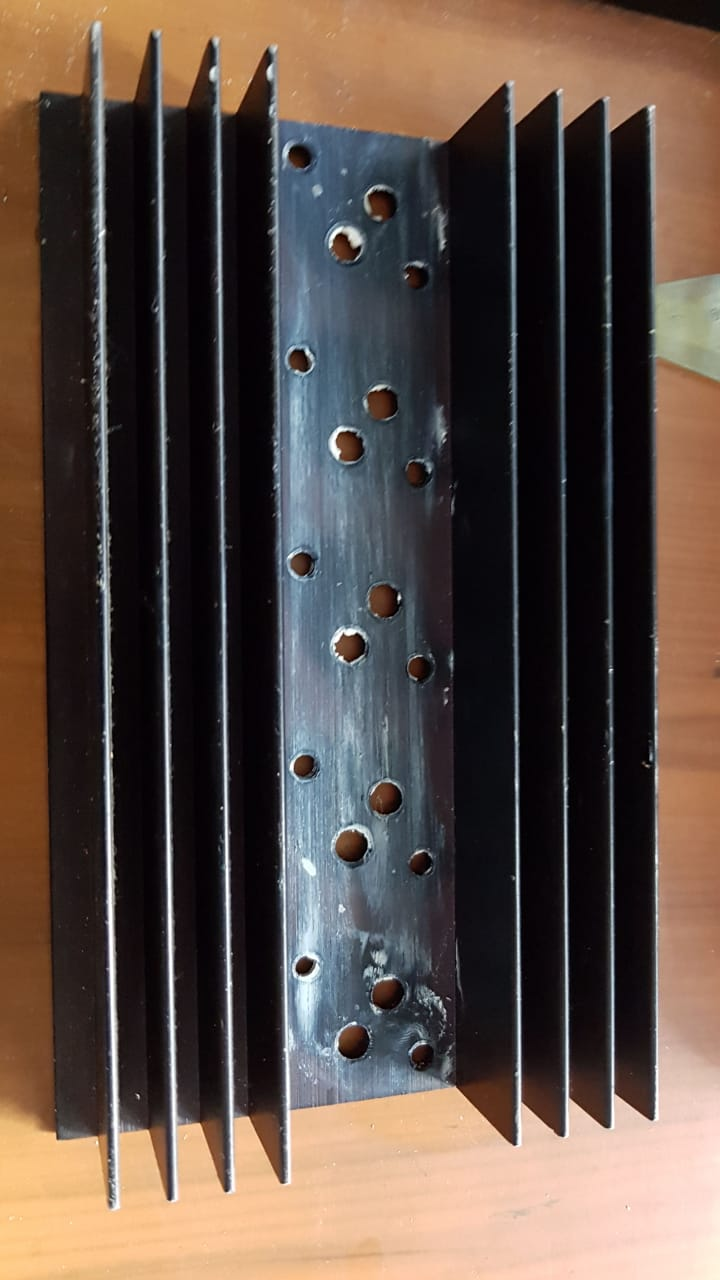
\includegraphics[angle=90,width=\linewidth]{disipador_seleccionado}
	\caption{disipador sobre el cual se montaran los transistores mosfet. Dada la situación actual, es el único disponible dentro de la institución}
\end{figure}



\section{Conclusiones}
En este trabajo, se expuso que el control sobre las llaves de un puente H tiene su complejidad. En él, se tuvieron que tener en cuentan todos los detalles en el aspecto teórico, desde la corriente máxima que circulará por él, potencia a disipar, resistencia de encendido, y temperatura. Todos estos aspectos, se fueron resolviendo de a uno en el presente capítulo, cada uno, presentando distintos grados de dificultad. Estos diseños, además, se han simulado con éxito, y no han presentado problemas a la hora de la simulación. Los resultados de la simulación se presentarán en el próximo informe en conjunto con el software final. Dado el estado de avance de proyecto, se espera, que el próximo informe de avance, contenga, además, los resultados, que en el presente informe no se han podido mostrar debido a la situación de la pandemia. En el próximo informe, se espera poder ir al IAR, a poder realizar medidas sobre la antena, así como el control y su movimiento. Si esto ocurre con éxito, se dará por finalizado el trabajo. 
